%% chapter13_slides.tex
%% Self-contained Beamer slides for
%% Chapter 13: Ship Routing and Scheduling in Industrial and Tramp Shipping
%% Source: Vehicle Routing: Problems, Methods, and Applications, 2nd ed., 2014
%% Authors: Marielle Christiansen, Kjetil Fagerholt
%%
%% Compile:  pdflatex -interaction=nonstopmode chapter13_slides.tex  (run twice)

\documentclass[aspectratio=169,10pt]{beamer}

\usetheme{Madrid}
\usecolortheme{seahorse}
\setbeamertemplate{footline}[frame number]
\setbeamertemplate{navigation symbols}{}

%% ── Packages ───────────────────────────────────────────────────────────────
\usepackage{amsmath,amssymb,amsthm}
\usepackage{mathtools}
\usepackage{graphicx}
\usepackage{booktabs}
\usepackage{array}
\usepackage{xcolor}
\usepackage{listings}
\usepackage{multicol}
\usepackage{tikz}
\usetikzlibrary{arrows.meta,shapes,positioning,fit,backgrounds}
\usepackage{pgfplots}
\pgfplotsset{compat=1.18}
\usepackage{microtype}
\usepackage{hyperref}

\graphicspath{{figures/}}

%% ── Listings style ─────────────────────────────────────────────────────────
\lstset{
  language=Python,
  basicstyle=\ttfamily\scriptsize,
  numbers=left,
  numberstyle=\tiny\color{gray},
  frame=single,
  backgroundcolor=\color{gray!7},
  commentstyle=\color{green!50!black}\itshape,
  keywordstyle=\color{blue!80!black}\bfseries,
  stringstyle=\color{red!70!black},
  breaklines=true,
  showstringspaces=false,
  tabsize=4,
}

%% ── Metadata ───────────────────────────────────────────────────────────────
\title[Ch.~13: Ship Routing]{Ship Routing and Scheduling\\
       in Industrial and Tramp Shipping}
\subtitle{Chapter 13 --- \textit{Vehicle Routing: Problems, Methods, and Applications},
          2nd~Edition (2014)}
\author{Marielle Christiansen \and Kjetil Fagerholt}
\institute{Lecture Notes --- Self-Contained Reading Version}
\date{2014}

%% ── Custom colours ─────────────────────────────────────────────────────────
\definecolor{ship_blue}{RGB}{21,101,192}
\definecolor{cargo_green}{RGB}{46,125,50}
\definecolor{tramp_orange}{RGB}{230,81,0}
\definecolor{highlight_yellow}{RGB}{255,249,196}
\definecolor{alert_red}{RGB}{198,40,40}

%%%%%%%%%%%%%%%%%%%%%%%%%%%%%%%%%%%%%%%%%%%%%%%%%%%%%%%%%%%%%%%%%%%%%%%%%%%
\begin{document}

\begin{frame}
  \titlepage
\end{frame}

%% ── Table of Contents ───────────────────────────────────────────────────────
\begin{frame}[allowframebreaks]{Chapter Overview}
  This chapter covers the rich family of ship routing and scheduling problems
  that arise in \textbf{industrial} and \textbf{tramp} maritime transportation.
  Unlike road vehicle routing, ship routing involves enormous cargo quantities,
  multi-week planning horizons, complex contractual arrangements, and
  variable fuel costs that depend on speed in a strongly non-linear way.

  \medskip
  \textbf{Topics covered in this chapter:}
  \begin{enumerate}
    \item \textbf{Introduction} --- the economic and environmental context of
          maritime shipping; the three main shipping segments.
    \item \textbf{Cargo Routing and Scheduling} --- the core optimisation
          problem for industrial and tramp shipping; exact and heuristic solution methods.
    \item \textbf{Maritime Inventory Routing (MIR)} --- integrating inventory
          management at ports with ship scheduling decisions.
    \item \textbf{Dynamic and Stochastic Ship Routing} --- handling weather
          uncertainty, port congestion, and real-time cargo spot offers.
    \item \textbf{Conclusions and Future Directions}.
  \end{enumerate}

  \medskip
  \begin{alertblock}{Key Takeaway of the Chapter}
    Maritime transportation is responsible for more than 80\% of world trade
    by volume.  Optimising ship routing and scheduling can reduce operational
    costs by 10--20\% and substantially cut CO$_2$ emissions, making this
    one of the most impactful application areas of vehicle routing research.
  \end{alertblock}
\end{frame}

%%%%%%%%%%%%%%%%%%%%%%%%%%%%%%%%%%%%%%%%%%%%%%%%%%%%%%%%%%%%%%%%%%%%%%%%%%%
\section{Introduction}
%%%%%%%%%%%%%%%%%%%%%%%%%%%%%%%%%%%%%%%%%%%%%%%%%%%%%%%%%%%%%%%%%%%%%%%%%%%

\begin{frame}[allowframebreaks]{Introduction: The Maritime Transportation Sector}
  International seaborne trade handles more than \textbf{8 billion tonnes} of
  goods annually (UNCTAD 2011), making maritime transport the backbone of
  global commerce.  Shipping is also a \emph{published} industry: to a
  published schedule, as in a bus service, or an \emph{ad-hoc} industry that
  follows the cargo wherever it goes.

  \medskip
  The sector is dominated by a small number of very large companies.
  Product tankers and bulk carriers --- the subjects of this chapter ---
  account for more than 60\% of shipping ton-miles.  These product
  carriers ship chemicals, petroleum products, liquefied gas, dry bulk
  commodities (grain, coal, ore), and other raw materials in quantities
  ranging from a few thousand to more than 300\,000 tonnes per voyage.

  \medskip
  \begin{block}{Three Shipping Segments}
    Maritime transport is traditionally divided into three segments:
    \begin{itemize}
      \item \textbf{Industrial shipping}: the shipowner controls both the
            fleet \emph{and} the cargo.  Routing and cargo decisions are
            made simultaneously (e.g., a mining company that owns its own
            bulk carriers).
      \item \textbf{Liner shipping}: ships operate on \emph{fixed, published
            schedules} (like a bus), visiting a set of ports in a regular
            rotation regardless of whether the ship is full.  The shipowner
            sells space on the ship (a slot) to individual shippers.
      \item \textbf{Tramp shipping}: the ship acts like a \emph{taxi} ---
            it follows the cargo.  The tramp operator bids on spot market
            cargoes and accepts long-term contracts, then optimises the
            fleet's routes to maximise profit.
    \end{itemize}
  \end{block}

  \begin{figure}
    \centering
    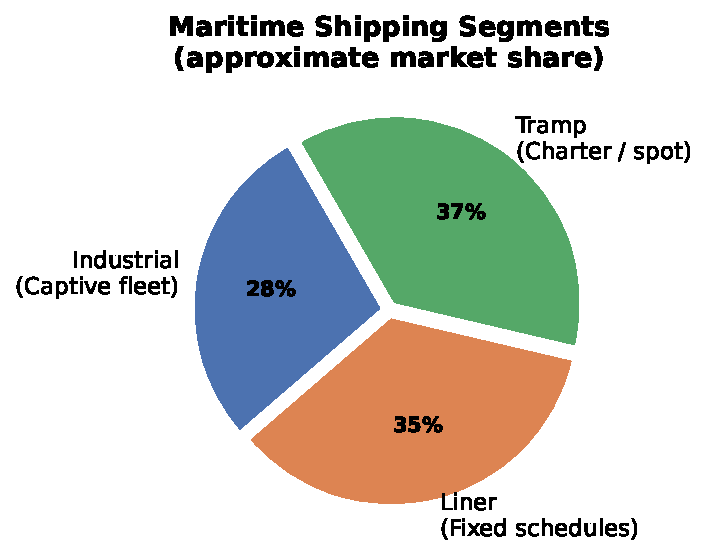
\includegraphics[width=0.62\textwidth]{shipping_segments.pdf}
    \caption{Approximate market share of the three maritime shipping segments.
             Industrial shipping involves vertically integrated firms;
             liner shipping is analogous to scheduled air transport;
             tramp shipping resembles a spot market (taxi) model.}
  \end{figure}

  \begin{exampleblock}{A Concrete Example of the Difference}
    Suppose a petroleum product (naphtha) needs to be moved from a refinery
    in Rotterdam to a chemical plant in Houston.
    \begin{itemize}
      \item An \textbf{industrial shipper} (e.g., Shell) that owns both the
            refinery and the destination plant would schedule one of its own
            product tankers to make the voyage.  Routing is an \emph{internal}
            decision.
      \item A \textbf{liner carrier} (e.g., Maersk) would take the cargo as
            a paying slot on its regular Atlantic service, which departs every
            two weeks regardless.
      \item A \textbf{tramp operator} would bid for the cargo on the spot
            market, assign whichever ship is most conveniently positioned,
            and negotiate the freight rate based on current supply and demand.
    \end{itemize}
  \end{exampleblock}

  \begin{figure}
    \centering
    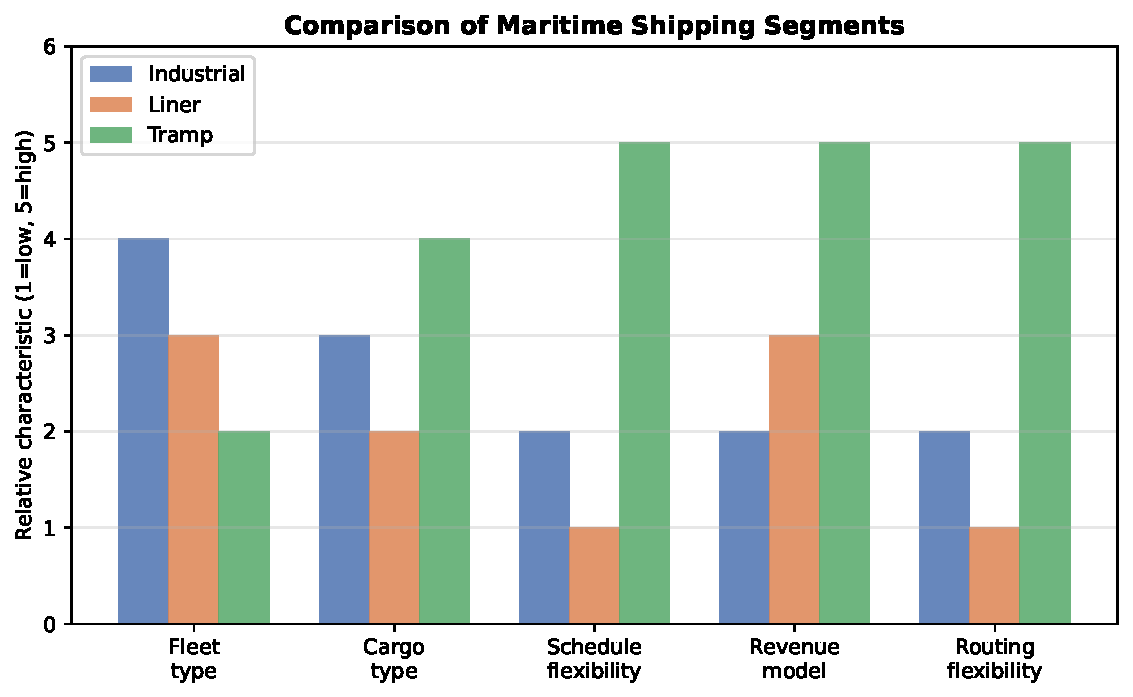
\includegraphics[width=0.70\textwidth]{segment_comparison.pdf}
    \caption{Radar-style comparison of the three shipping segments across
             five operational dimensions.  Tramp shipping scores highest on
             flexibility; liner shipping sacrifices flexibility for schedule
             reliability; industrial shipping integrates cargo and fleet
             management.}
  \end{figure}

  \begin{alertblock}{Why Optimisation Matters}
    Operating a fleet of product tankers costs tens of millions of USD per year.
    Fuel alone accounts for 50--70\% of voyage costs, and fuel consumption
    scales as the \emph{cube} of ship speed.  A 10\% reduction in average speed
    reduces fuel consumption by about 27\%.  Optimising routes and speed
    profiles therefore has enormous economic and environmental impact.
    According to \cite{Vidal2007}, shipping produces twice as much CO$_2$
    as aviation; this makes efficient ship routing a pressing sustainability
    challenge.
  \end{alertblock}
\end{frame}

%%%%%%%%%%%%%%%%%%%%%%%%%%%%%%%%%%%%%%%%%%%%%%%%%%%%%%%%%%%%%%%%%%%%%%%%%%%
\section{Cargo Routing and Scheduling}
%%%%%%%%%%%%%%%%%%%%%%%%%%%%%%%%%%%%%%%%%%%%%%%%%%%%%%%%%%%%%%%%%%%%%%%%%%%

\begin{frame}[allowframebreaks]{Section 13.2: Cargo Routing and Scheduling}
  This section covers the core problem of \textbf{routing a heterogeneous
  fleet of ships to serve a set of cargoes}.  The problem arises in both
  industrial and tramp shipping contexts and is fundamentally a
  \emph{pickup-and-delivery} vehicle routing problem on a maritime network.

  \medskip
  Unlike classical road VRP, the maritime pickup-and-delivery problem has
  several distinctive features:
  \begin{enumerate}
    \item Cargo quantities are very large (thousands of tonnes), and a
          single ship may carry only \emph{one} cargo at a time (full
          ship-load) or several smaller cargoes simultaneously.
    \item Some cargoes are \textbf{mandatory} (long-term contracts that
          \emph{must} be served); others are \textbf{optional} (spot market
          cargoes that can be declined at a cost, or served by a chartered
          ``spot market'' ship at a fixed fee).
    \item The planning horizon is typically \emph{weeks to months}, not hours.
    \item Each ship has its own \emph{origin} (current position) and an
          \emph{artificial destination} representing the end of its planning
          period.
    \item Time windows are specified at each port for both loading and
          discharging, often with \emph{hard} windows (no wait outside the
          window is allowed at the terminal).
  \end{enumerate}
\end{frame}

%% ─────────────────────────────────────────────────────────────────────────
\subsection{13.2.1 Maritime Pickup-and-Delivery}
%% ─────────────────────────────────────────────────────────────────────────

\begin{frame}[allowframebreaks]{The Maritime Pickup-and-Delivery Problem (MPDP)}
  \begin{block}{Problem Definition}
    We are given a fleet $K$ of ships and a set $N^C$ of \emph{mandatory
    cargoes} together with a set $N^O$ of \emph{optional} (spot-market)
    cargoes.  Each cargo $i$ has a pickup port and a delivery port, a
    quantity $Q_i$ (tonnes), and a revenue $R_i$ per unit transported.
    The goal is to assign cargoes to ships and determine each ship's route
    and schedule to \textbf{maximise profit} (revenue minus voyage costs).
  \end{block}

  \medskip
  \textbf{Network structure.} For each ship $k \in K$ we build a directed
  graph.  Let $N_k^P$ denote the set of \emph{pickup} nodes for ship $k$
  (one per cargo that ship $k$ could potentially carry), and let $N_k^D$
  be the corresponding \emph{delivery} nodes.  In addition, each ship $k$
  has an artificial \emph{origin} node $o(k)$ (its current location at the
  start of the planning period) and an artificial \emph{destination} node
  $d(k)$ (representing ``done'').

  \medskip
  \begin{block}{Notation (read carefully)}
    \begin{itemize}
      \item $K$ --- the set of all ships in the fleet.
      \item $N^C$ --- set of \textbf{mandatory} cargo indices (contracts).
      \item $N^O$ --- set of \textbf{optional} (spot market) cargo indices.
      \item $N_k = N_k^P \cup N_k^D \cup \{o(k), d(k)\}$ --- all nodes
            relevant to ship $k$.
      \item $A_k$ --- set of \textbf{arcs} (pairs of nodes) for ship $k$;
            an arc $(i,j) \in A_k$ means ship $k$ can sail directly from
            node $i$ to node $j$.
      \item $Q_i$ --- the \textbf{quantity} (load in tonnes) of cargo $i$.
      \item $Q_k^C$ --- the \textbf{capacity} (maximum load in tonnes) of
            ship $k$.
      \item $R_i$ --- the \textbf{revenue} earned per tonne of cargo $i$
            transported.
      \item $C_{ijk}$ --- the \textbf{voyage cost} for ship $k$ to sail
            from node $i$ to node $j$ (fuel, port fees, canal tolls, etc.).
      \item $C_i^S$ --- the \textbf{spot market cost} --- the fee paid to
            hire an outside ship to carry mandatory cargo $i$ if none of
            our ships can.
    \end{itemize}
  \end{block}

  \begin{block}{Decision Variables}
    \begin{itemize}
      \item $x_{ijk} \in \{0, 1\}$ (``x sub $i$-$j$-$k$'') --- equals 1 if
            ship $k$ sails \emph{directly} from node $i$ to node $j$, and 0
            otherwise.
      \item $z_i \in \{0, 1\}$ --- equals 1 if mandatory cargo $i \in N^C$
            is served by a \emph{spot market} ship (not by our own fleet).
      \item $y_i \in \{0, 1\}$ --- equals 1 if optional cargo $i \in N^O$ is
            actually transported (accepted and loaded), 0 if declined.
      \item $t_{ik} \geq 0$ --- the \textbf{time} at which ship $k$ begins
            service at node $i$.
      \item $l_{ik} \geq 0$ --- the \textbf{load} (weight in tonnes) on ship
            $k$ when it \emph{departs} from node $i$.
    \end{itemize}
  \end{block}
\end{frame}

\begin{frame}[allowframebreaks]{The MPDP Mathematical Model (Equations 13.1--13.15)}
  The tramp ship routing and scheduling problem can now be written as a
  \textbf{Mixed-Integer Programme (MIP)}.  We state each constraint
  group in turn and explain what it enforces.

  \medskip
  \begin{block}{Objective Function (13.1) --- Maximise Profit}
    \begin{equation}
      \max \; \underbrace{\sum_{i \in N^C} R_i Q_i}_{\text{mandatory revenue}}
           + \underbrace{\sum_{i \in N^O} R_i Q_i y_i}_{\text{optional revenue}}
           - \underbrace{\sum_{k \in K} \sum_{(i,j) \in A_k} C_{ijk} x_{ijk}}_{\text{voyage costs}}
           - \underbrace{\sum_{i \in N^C} C_i^S z_i}_{\text{spot market cost}}
      \tag{13.1}
    \end{equation}
  \end{block}

  The objective function adds revenue from \emph{all} mandatory cargoes
  (because they must be carried, either by our fleet or by a spot ship),
  plus revenue from optional cargoes we choose to carry, then subtracts
  the total voyage cost of our fleet and the cost of any spot market ships
  hired to cover mandatory cargoes we cannot serve ourselves.

  \medskip
  \begin{alertblock}{How to Read This Objective}
    Think of the formula as a \emph{net profit} calculation.  The first two
    terms are gross revenue; the last two are costs.  Hiring a spot ship
    (term $C_i^S z_i$) is expensive, so the solver prefers to assign
    mandatory cargoes to own ships.  However, if a mandatory cargo is
    geographically inconvenient, paying the spot premium may still be
    optimal.  Optional cargoes are only accepted if they generate more
    revenue than the additional voyage cost they impose.
  \end{alertblock}

  \bigskip
  \textbf{Constraint (13.2) --- Every mandatory cargo is served:}
  \begin{equation}
    \sum_{k \in K} \sum_{j \in N_k} x_{ijk} + z_i = 1
    \qquad \forall\, i \in N^C
    \tag{13.2}
  \end{equation}
  This constraint says: for each mandatory cargo $i$, either one of our
  ships picks it up (the left double-sum equals 1) \emph{or} the spot
  market covers it ($z_i = 1$).  The sum of the two alternatives must
  equal exactly 1, ensuring the cargo is not served twice and not missed.

  \medskip
  \textbf{Constraint (13.3) --- Optional cargo:}
  \begin{equation}
    \sum_{k \in K} \sum_{j \in N_k} x_{ijk} - y_i = 0
    \qquad \forall\, i \in N^O
    \tag{13.3}
  \end{equation}
  For optional cargo $i$: the indicator $y_i = 1$ if and only if some ship
  actually picks it up.  If no ship visits the pickup node ($\sum x_{ijk}=0$),
  then $y_i = 0$ and the cargo is simply not carried.

  \medskip
  \textbf{Constraint (13.4) --- Each ship departs its origin exactly once:}
  \begin{equation}
    \sum_{j \in N_k} x_{o(k)jk} = 1 \qquad \forall\, k \in K
    \tag{13.4}
  \end{equation}

  \textbf{Constraint (13.5) --- Flow conservation (no teleportation):}
  \begin{equation}
    \sum_{j \in N_k} x_{ijk} - \sum_{j \in N_k} x_{jik} = 0
    \qquad \forall\, k \in K,\;
    i \in N_k \setminus \{o(k), d(k)\}
    \tag{13.5}
  \end{equation}
  For every intermediate node $i$ (not origin or destination), the number
  of times ship $k$ \emph{arrives} at $i$ equals the number of times it
  \emph{departs} from $i$.  This prevents ``disappearing ships.''

  \medskip
  \textbf{Constraint (13.6) --- Each ship arrives at its destination:}
  \begin{equation}
    \sum_{i \in N_k} x_{id(k)k} = 1 \qquad \forall\, k \in K
    \tag{13.6}
  \end{equation}

  \textbf{Constraint (13.7) --- Load increases at pickup:}
  \begin{equation}
    l_{ik} + Q_j - l_{jk} - Q_k^C (1 - x_{ijk}) \leq 0
    \qquad \forall\, k \in K,\; (i,j) \in A_k,\; j \in N_k^P
    \tag{13.7}
  \end{equation}
  Here $l_{ik}$ (l sub $i$-$k$) is the load \emph{after} departing node $i$.
  At a pickup node $j$, the load increases by $Q_j$.  If ship $k$ does
  \emph{not} travel arc $(i,j)$ (i.e., $x_{ijk}=0$), the ``big-M'' term
  $Q_k^C$ relaxes this constraint to a trivial upper bound, ensuring it only
  applies on arcs actually used.

  \textbf{Constraint (13.8) --- Load decreases at delivery:}
  \begin{equation}
    l_{ik} - Q_j - l_{n+j,k} - Q_k^C (1 - x_{i,n+j,k}) \leq 0
    \qquad j \in N_k^P
    \tag{13.8}
  \end{equation}
  At a delivery node (indexed $n+j$), the load decreases by $Q_j$.  The
  index $n+j$ refers to the delivery node associated with pickup node $j$
  (pickup nodes are indexed $1\ldots n$, delivery nodes $n+1\ldots 2n$).

  \medskip
  \textbf{Constraint (13.9) --- Capacity at pickup:}
  \begin{equation}
    \sum_{j \in N_k} Q_i x_{ijk} \leq l_{ik}
      \leq \sum_{j \in N_k} Q_k^C x_{ijk}
    \qquad \forall\, k \in K,\; i \in N_k^P
    \tag{13.9}
  \end{equation}
  The load on ship $k$ must stay between the quantity of the cargo just
  loaded ($Q_i$) and the ship's full capacity $Q_k^C$.

  \medskip
  \textbf{Constraints (13.10)--(13.12) --- Time-window feasibility:}
  These constraints enforce that ship $k$ arrives at each node within the
  allowed time window $[\underline{T}_{ik},\, \overline{T}_{ik}]$.
  Constraint (13.11) ensures that the time spent at node $i$ is at least
  $T_{ik}^P$ (port handling time).  The big-M formulation links arrival
  times to route decisions via the binary $x_{ijk}$ variables.

  \begin{block}{Time window notation}
    $\underline{T}_{ik}$ (T sub $i$-$k$, underlined = \emph{lower} bound)
    is the \emph{earliest} time ship $k$ may begin service at node $i$.
    $\overline{T}_{ik}$ (T sub $i$-$k$, overlined = \emph{upper} bound) is
    the \emph{latest} time.  $T_{ijk}^S$ is the sailing time from node $i$
    to node $j$ for ship $k$.  $M_{ijk}$ is a sufficiently large constant
    (``big-M'') used to activate/deactivate a constraint based on
    whether arc $(i,j)$ is used.
  \end{block}

  \begin{figure}
    \centering
    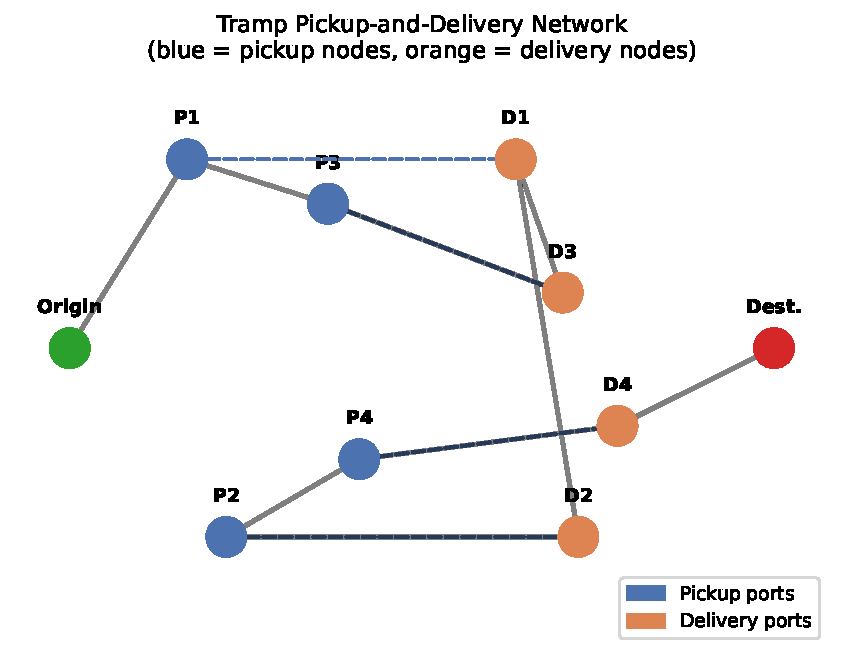
\includegraphics[width=0.7\textwidth]{tramp_network.pdf}
    \caption{A tramp ship pickup-and-delivery network.  Blue circles are
             pickup ports (where the ship loads cargo); orange circles are
             delivery ports (where the ship unloads).  The ship starts at
             Origin and must reach Destination (artificial end node).
             The black path shows one feasible route through all four
             cargo pairs.}
  \end{figure}
\end{frame}

%% ─────────────────────────────────────────────────────────────────────────
\subsection{Split Loads}
%% ─────────────────────────────────────────────────────────────────────────

\begin{frame}[allowframebreaks]{13.2.1 Extension: Split Loads}
  In the standard formulation above, each cargo is assigned to
  \emph{exactly one} ship.  However, when cargo quantities exceed any
  single ship's capacity, or when using two ships would allow a faster
  (and therefore more profitable) delivery, it may be advantageous to
  \textbf{split a cargo across multiple ships}.

  \medskip
  \begin{block}{What Split Loads Mean}
    Suppose cargo $i$ has quantity $Q_i = 80{,}000$ tonnes but every ship in
    the fleet has capacity $Q_k^C = 50{,}000$ tonnes.  Without splitting, the
    cargo simply cannot be served by the fleet.  With \emph{split loads}, two
    ships each carry a fraction: say Ship~1 carries 50\,000 tonnes and Ship~2
    carries 30\,000 tonnes, both picking up at the same port and delivering at
    the same destination.
  \end{block}

  When split loads are allowed, additional continuous variables $q_{ijk}$
  representing the \emph{quantity} carried by ship $k$ on arc $(i,j)$ for
  cargo $i$ are introduced, together with pairing constraints that ensure
  the total quantity carried across all ships and all arcs sums to $Q_i$.

  \begin{figure}
    \centering
    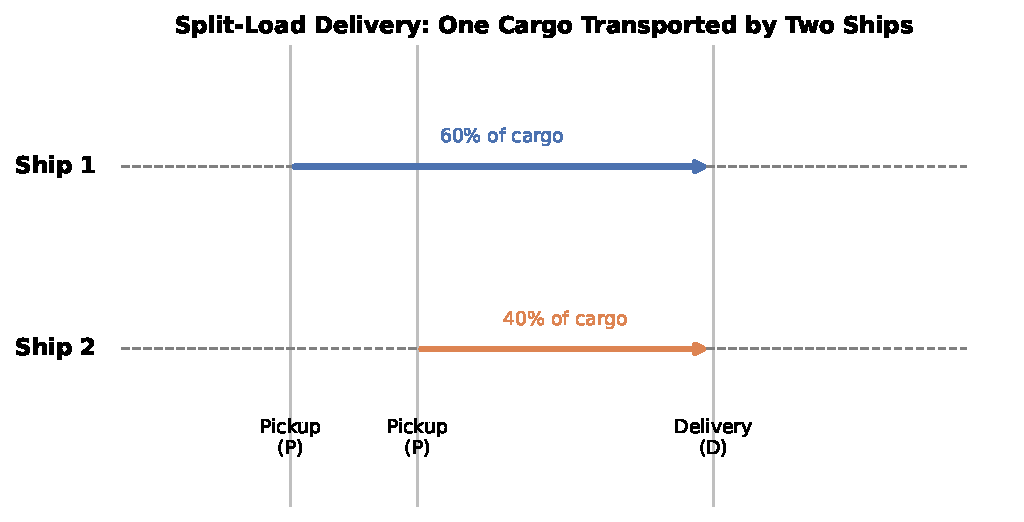
\includegraphics[width=0.70\textwidth]{split_loads.pdf}
    \caption{Split-load delivery: a single cargo is divided between two ships.
             Ship~1 carries 60\% and Ship~2 carries 40\% of the total quantity.
             Both ships pick up at the same port (marked ``Pickup P'') and
             deliver to the same destination (``Delivery D'').}
  \end{figure}

  \begin{exampleblock}{Worked Example: When Does Splitting Help?}
    Suppose we have two cargoes and two ships, each with capacity 50 units:
    \begin{itemize}
      \item Cargo A: pickup at port 1, delivery at port 2, quantity = 70 units.
      \item Cargo B: pickup at port 3, delivery at port 4, quantity = 30 units.
    \end{itemize}
    \textbf{Without splitting}: Cargo A (70 units) cannot fit on any single ship
    (capacity = 50), so a spot ship must be hired at high cost.
    \textbf{With splitting}: Ship~1 takes 50 units of Cargo A; Ship~2 takes the
    remaining 20 units of Cargo A and all 30 units of Cargo B.  Both constraints
    are satisfied and no spot ship is needed.

    The key insight is that split loads significantly expand the set of feasible
    solutions, especially for bulk products where cargo sizes can be large.
  \end{exampleblock}

  \begin{alertblock}{References}
    St\aa lhane et al.\ (2012) develop a branch-and-cut algorithm for the
    ship routing and scheduling problem \emph{with split loads}.
    Their branch-and-cut outperforms a direct MIP solver on instances with
    up to 30 cargoes and 6 ships.
  \end{alertblock}
\end{frame}

%% ─────────────────────────────────────────────────────────────────────────
\subsection{Variable Speed}
%% ─────────────────────────────────────────────────────────────────────────

\begin{frame}[allowframebreaks]{13.2.2 Application-Driven Modelling: Variable Sailing Speed}
  Real-world ship routing involves a powerful lever unavailable in road VRP:
  the ship's operator can \textbf{freely choose speed} on each leg.
  This matters because the relationship between speed and fuel consumption
  is strongly non-linear.

  \medskip
  \begin{block}{The Cubic Fuel Consumption Law}
    Let $v$ (v, for velocity in knots, where 1 knot $\approx 1.85$ km/h) be
    the speed of a ship on a particular leg.  The fuel consumption rate
    $F(v)$ (in tonnes per day) is approximately:
    \begin{equation}
      F(v) \;=\; \alpha \cdot v^3
    \end{equation}
    where $\alpha$ (alpha) is a ship-specific constant (depending on hull
    form, engine efficiency, etc.).  This cubic relationship means:
    reducing speed by 10\% reduces fuel consumption by approximately
    $1 - 0.9^3 \approx 27\%$.
  \end{block}

  \begin{alertblock}{How to Read This Formula}
    If you double the speed, fuel consumption increases \emph{eightfold}
    ($2^3 = 8$).  This is why ``slow steaming'' --- operating well below
    design speed --- has been adopted industry-wide since fuel price spikes
    in the 2000s.  The trade-off is that slower ships spend more time at
    sea, which may miss time windows or require more ships to maintain
    the same throughput.
  \end{alertblock}

  \begin{figure}
    \centering
    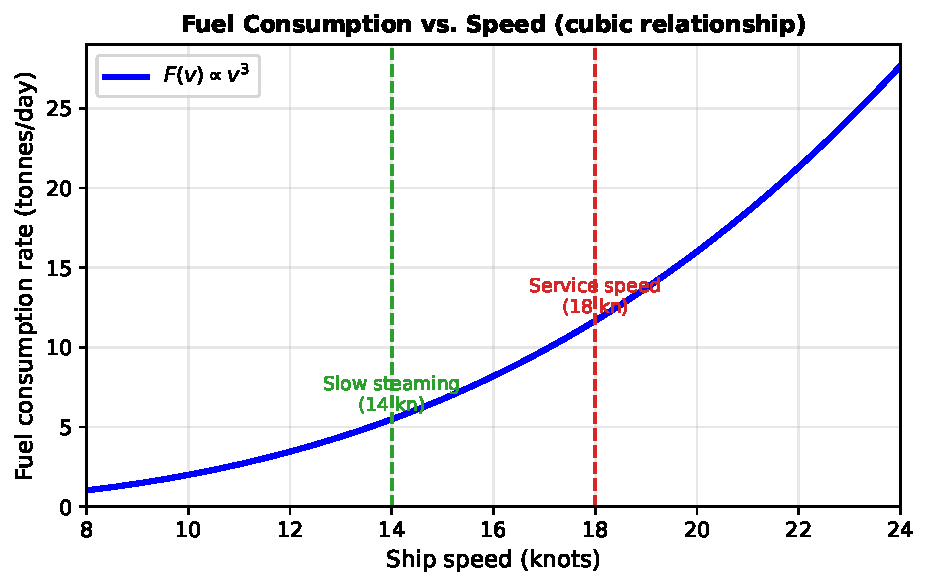
\includegraphics[width=0.60\textwidth]{variable_speed.pdf}
    \caption{Fuel consumption rate $F(v) = \alpha \cdot v^3$ as a function
             of ship speed $v$ in knots.  At the ``slow steaming'' speed
             of 14 knots versus the service speed of 18 knots, fuel
             consumption is reduced by $1-(14/18)^3 \approx 40\%$.
             This represents a very large cost saving per voyage.}
  \end{figure}

  \medskip
  \textbf{Modelling variable speed.}  When speed can be optimised, the
  total cost of a voyage from node $i$ to node $j$ for ship $k$ is:
  \begin{equation}
    C_{ijk}(v) \;=\; \alpha_k \cdot v^3 \cdot \frac{d_{ij}}{v}
                \;=\; \alpha_k \cdot d_{ij} \cdot v^2
  \end{equation}
  where $d_{ij}$ is the distance in nautical miles, $v$ is the sailing speed,
  and the formula converts from ``rate per unit time'' to ``total fuel over
  the leg.''  Crucially, choosing speed $v$ also determines transit time
  $d_{ij}/v$, which affects time-window feasibility.  The optimisation must
  simultaneously determine \emph{routes} and \emph{speeds}.

  \begin{block}{Papageorgiou and Kannan (2015) --- Speed Optimisation Model}
    Panaitescu and Rutenberg \cite{Fagerholt2010} showed that the variable
    speed model (13.16)--(13.18) replaces the fixed cost $C_{ijk}$ in the
    objective (13.1) with a quadratic term in $v$.  The resulting formulation
    is a \textbf{Mixed-Integer Non-Linear Programme (MINLP)}, which is harder
    to solve but captures real-world costs much more accurately.
    For large instances, Fagerholt et al.\ (2010) propose a network
    flow heuristic that reduces the MINLP to a sequence of linear
    sub-problems, allowing near-optimal solutions for fleets of 15--20 ships.
  \end{block}

  \begin{exampleblock}{Numerical Example: Speed--Cost Trade-off on One Leg}
    Suppose ship $k$ must sail from Rotterdam to Houston, a distance of
    $d = 7{,}800$ nautical miles.  The ship's engine constant is
    $\alpha_k = 0.002$ (tonnes of fuel per day per knot$^3$).
    Fuel costs \$600 per tonne.

    \medskip
    \textbf{At 18 knots (design speed):}
    Transit time $= 7800/18 \approx 433$ hours $= 18.1$ days.
    Fuel used $= 0.002 \times 18^3 \times 18.1 = 0.002 \times 5832 \times 18.1
    \approx 211$ tonnes.
    Fuel cost $= 211 \times 600 \approx \$126{,}600$.

    \medskip
    \textbf{At 14 knots (slow steaming):}
    Transit time $= 7800/14 \approx 557$ hours $= 23.2$ days.
    Fuel used $= 0.002 \times 14^3 \times 23.2 = 0.002 \times 2744 \times 23.2
    \approx 127$ tonnes.
    Fuel cost $= 127 \times 600 \approx \$76{,}200$.

    \textbf{Saving $\approx \$50{,}000$ per voyage} simply by sailing slower,
    at the cost of 5.1 extra days at sea.
  \end{exampleblock}
\end{frame}

%% ─────────────────────────────────────────────────────────────────────────
\subsection{Solution Methods for MPDP}
%% ─────────────────────────────────────────────────────────────────────────

\begin{frame}[allowframebreaks]{Solution Methods: Exact Approaches}
  The MPDP is NP-hard (it subsumes the TSP), so exact algorithms can
  only solve instances of moderate size.  Two main exact approaches appear
  in the literature.

  \medskip
  \begin{block}{Branch-and-Bound (B\&B)}
    The standard MIP formulation (13.1)--(13.15) can be solved directly by
    an off-the-shelf MIP solver (e.g., CPLEX or Gurobi) using
    \textbf{branch-and-bound}.  The solver relaxes the integrality
    constraints on $x_{ijk}$, solves the LP relaxation, then
    \textbf{branches} on a fractional variable (fixes it to 0 or 1 in two
    sub-problems) and recursively solves each sub-problem.  Valid
    \textbf{inequalities} (cuts) are added to tighten the LP bound.

    For ship routing, the fleet is typically heterogeneous (ships differ in
    speed, capacity, and fuel efficiency), and the number of cargoes can
    reach 40--60 in real planning instances.  Direct B\&B solves instances
    with up to about 30 cargoes and 5--6 ships within an hour.
  \end{block}

  \begin{block}{Branch-and-Price (B\&P)}
    A more powerful exact method is \textbf{branch-and-price}, which combines
    branch-and-bound with \textbf{column generation}.  Instead of enumerating
    all possible arcs $x_{ijk}$ (which grow exponentially with the number
    of ports), the master problem works with \emph{complete ship routes}
    (sequences of nodes) as columns.

    \begin{enumerate}
      \item The \textbf{Restricted Master Problem (RMP)} selects the best
            subset of routes from a current (small) pool; its LP relaxation
            yields dual prices $\pi_i$ for each cargo coverage constraint.
      \item The \textbf{Pricing Subproblem} (one per ship) finds the route
            with the most negative \emph{reduced cost}:
            $\bar{c}_r = c_r - \sum_{i} \pi_i a_{ir}$,
            where $a_{ir} = 1$ if route $r$ covers cargo $i$.
            This is typically solved as a shortest-path problem on a
            time-expanded graph.
      \item If a route with $\bar{c}_r < 0$ is found, it is added to the
            RMP as a new column and the process repeats.
      \item When no improving column exists, the LP relaxation is optimal;
            branching enforces integrality.
    \end{enumerate}

    B\&P can solve instances with 40--80 cargoes because it only ever
    handles a polynomial number of routes at any time.
  \end{block}

  \begin{figure}
    \centering
    
\includegraphics[width=0.60\textwidth]{branch_price.pdf}
    \caption{Schematic of the Branch-and-Price algorithm.  Column generation
             at each node of the branch-and-bound tree generates only
             ``useful'' ship routes (those with negative reduced cost),
             dramatically reducing the search space compared with
             enumerating all possible routes in advance.}
  \end{figure}

  \begin{alertblock}{Key Insight: Why Column Generation Works}
    The number of feasible ship routes is \emph{exponentially large}
    (it grows factorially with the number of ports).  Column generation
    avoids enumerating all routes by asking: ``Given the current LP solution,
    which route would most improve the objective?''  This is answered by
    solving a \emph{shortest-path subproblem} with time windows and
    capacity constraints --- a tractable sub-problem that generates
    only the routes the master problem actually needs.
  \end{alertblock}
\end{frame}

\begin{frame}[allowframebreaks]{Solution Methods: Heuristic Approaches}
  For large real-world instances (more than 50 cargoes, more than 10 ships),
  exact methods are too slow.  The chapter describes several powerful
  heuristics.

  \medskip
  \begin{block}{Tabu Search (TS)}
    Tabu search is a \textbf{local search metaheuristic} that systematically
    explores the neighbourhood of the current solution, accepting moves
    that improve the objective, but also allowing temporary ``uphill'' moves
    to escape local optima.

    The name ``tabu'' (from the Polynesian word for ``forbidden'') refers to
    a \emph{tabu list} that records recently visited moves.  A move is
    forbidden if it reverses a recently made change, preventing the algorithm
    from cycling back to the same solution.

    In ship routing, a \textbf{neighbourhood} is defined by operators such as:
    \begin{itemize}
      \item \textbf{Reinsertion}: remove cargo $i$ from ship $k$'s route and
            reinsert it into ship $k'$'s route (or hire a spot ship).
      \item \textbf{Swap}: exchange cargo $i$ on ship $k$ with cargo $j$ on ship $k'$.
      \item \textbf{2-opt within a ship}: reverse a sub-sequence of ports
            on the same ship's route.
    \end{itemize}
    Christiansen, Fagerholt, and Ronen \cite{CFR2004} apply TS to a
    real-world tramp problem and show that it achieves solutions within
    2--5\% of the optimum for instances that exact methods cannot solve.
  \end{block}

  \begin{figure}
    \centering
    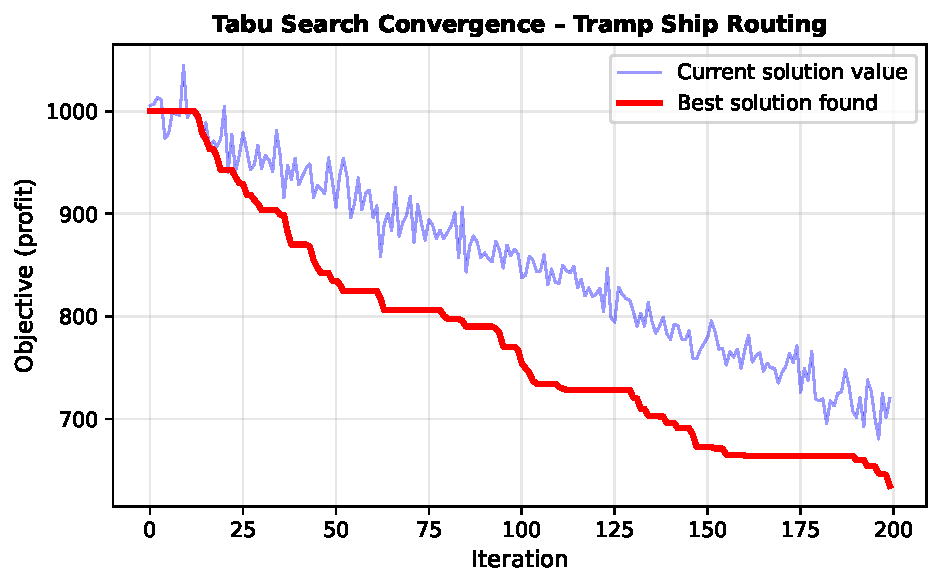
\includegraphics[width=0.55\textwidth]{tabu_convergence.pdf}
    \caption{Typical tabu search convergence for a tramp ship routing
             instance.  The blue line shows the current solution value
             (which can move uphill, i.e., worsen temporarily); the red line
             tracks the \emph{best} solution found so far.  Note how the
             algorithm escapes several local optima before finding the final
             best.}
  \end{figure}

  \begin{block}{Adaptive Large Neighbourhood Search (ALNS)}
    ALNS extends tabu search by using multiple \emph{destroy-and-repair}
    operators, selecting the most effective one adaptively based on recent
    performance.  The destroy phase removes a subset of cargoes from their
    current ship assignments; the repair phase reinserts them using a
    greedy or regret-based heuristic.

    ALNS has been shown to outperform single-neighbourhood TS on the
    MPDP, especially when the instance has a mix of mandatory and optional
    cargoes that require different reinsertion strategies.
  \end{block}

  \begin{exampleblock}{Greedy Insertion for MPDP (Illustrative Algorithm)}
    \textbf{Algorithm: Greedy Construction Heuristic for Tramp MPDP}
    \begin{enumerate}
      \item \textbf{Initialise}: assign each mandatory cargo $i \in N^C$ to
            the cheapest feasible ship $k^*$ (ignoring other cargoes).
      \item \textbf{Rank optional cargoes} by profitability ratio
            $R_i Q_i / C_i^{\text{marginal}}$ in decreasing order,
            where $C_i^{\text{marginal}}$ is the extra voyage cost of
            inserting cargo $i$ into the best available ship route.
      \item \textbf{For each optional cargo} $i$ in ranked order:
            compute the cheapest feasible insertion position across all
            ships.  If insertion increases profit, accept it.
      \item \textbf{For unserved mandatory cargoes}: assign a spot ship
            at cost $C_i^S$.
      \item \textbf{Return} the constructed solution.
    \end{enumerate}
    This greedy heuristic typically provides a feasible starting solution
    within a few minutes, which can then be improved by TS or ALNS.
  \end{exampleblock}
\end{frame>

%% ─────────────────────────────────────────────────────────────────────────
\subsection{Other Extensions: Liner Shipping}
%% ─────────────────────────────────────────────────────────────────────────

\begin{frame}[allowframebreaks]{13.2.2 Other Extensions: Liner Shipping and Multi-Commodity}
  The chapter also surveys extensions beyond the basic MPDP:

  \medskip
  \begin{block}{Liner Shipping Network Design}
    In liner shipping, the goal is to design \textbf{fixed weekly rotation
    loops} that minimise the cost of transporting all forecast demand between
    port pairs.  Unlike tramp shipping, the ship visits the same sequence
    of ports week after week (the ``string'').  The problem is:

    \begin{enumerate}
      \item \textbf{Select which ports} to include in each service loop.
      \item \textbf{Determine the frequency} (e.g., weekly or bi-weekly).
      \item \textbf{Decide how many ships} to deploy on each loop.
      \item \textbf{Route individual containers} (multiple commodities)
            across multiple overlapping loops using transshipment.
    \end{enumerate}

    This is sometimes called the \textbf{Liner Shipping Network Design
    Problem (LSNDP)}.  It is significantly more complex than the tramp MPDP
    because it involves a \emph{strategic} planning decision (the loop
    structure) on top of the operational routing decision.
  \end{block}

  \begin{figure}
    \centering
    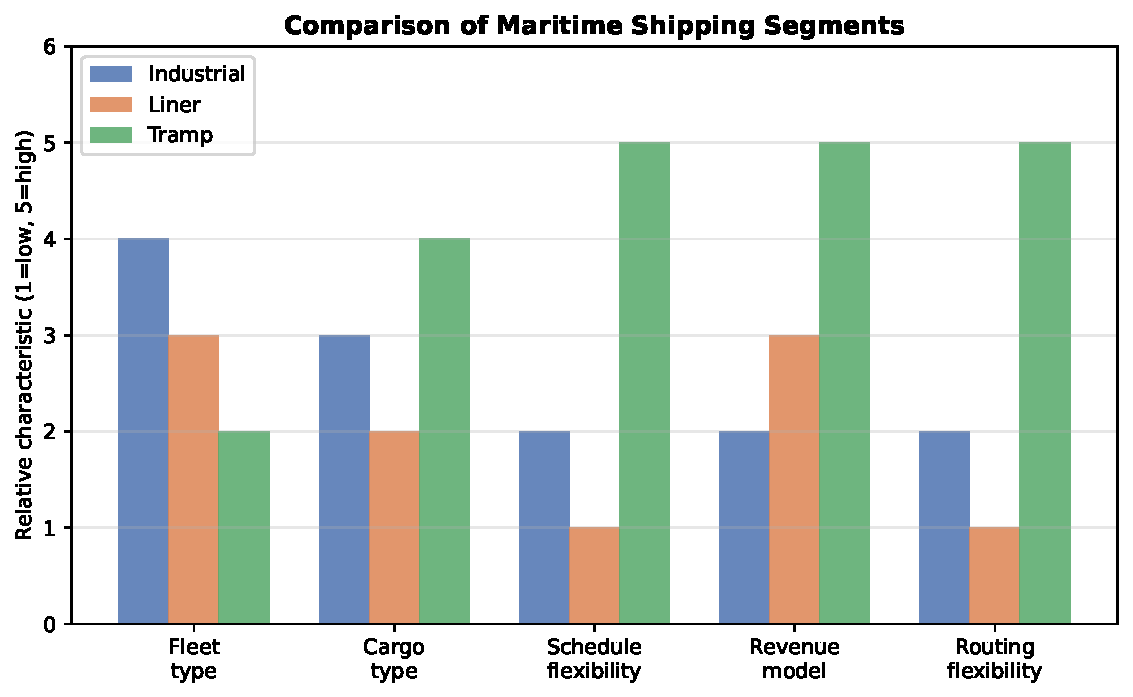
\includegraphics[width=0.55\textwidth]{segment_comparison.pdf}
    \caption{Comparison of the three shipping segments.  Liner shipping
             has the lowest scheduling flexibility (fixed rotations) but
             the highest schedule reliability from the shipper's perspective.}
  \end{figure}

  \begin{block}{Multi-Commodity (Multiple-Product) Ships}
    Some product tankers are partitioned into several \textbf{compartments},
    allowing them to carry different products simultaneously.  For example,
    a chemical tanker might carry naphtha in one tank and methanol in
    another.  This introduces:
    \begin{itemize}
      \item A \textbf{compartment assignment} sub-problem: which product
            goes in which tank?
      \item \textbf{Cleaning constraints}: switching from one chemical to
            another requires tank cleaning, which takes time and costs money.
      \item A more complex load-tracking model, since loads must be tracked
            per product, not just in aggregate.
    \end{itemize}
    Siswanto, Essam, and Sarker (2011) develop a MIP model and metaheuristic
    for this multi-compartment variant.
  \end{block}

  \begin{alertblock}{Takeaway for Cargo Routing and Scheduling}
    The basic MPDP formulation (13.1)--(13.15) captures the essential
    trade-off between revenue from optional cargoes, cost of serving
    mandatory cargoes, and fleet utilisation.  Extensions for split loads,
    variable speed, and multiple compartments make the problem harder but
    more realistic.  Exact methods (B\&P) solve medium-size instances;
    ALNS and tabu search handle large real-world fleets.
  \end{alertblock}
\end{frame>

%%%%%%%%%%%%%%%%%%%%%%%%%%%%%%%%%%%%%%%%%%%%%%%%%%%%%%%%%%%%%%%%%%%%%%%%%%%
\section{Maritime Inventory Routing}
%%%%%%%%%%%%%%%%%%%%%%%%%%%%%%%%%%%%%%%%%%%%%%%%%%%%%%%%%%%%%%%%%%%%%%%%%%%

\begin{frame}[allowframebreaks]{Section 13.3: Maritime Inventory Routing (MIR)}
  Maritime Inventory Routing (MIR) integrates \textbf{inventory management
  at ports} with \textbf{ship scheduling}.  Instead of treating cargoes as
  discrete units (as in MPDP), MIR thinks of the supply chain as a
  continuous flow: production facilities generate stock; consumption
  facilities draw down stock; ships shuttle material between them.
  The operator must ensure that no facility \emph{runs out of stock}
  (a ``stock-out'') or \emph{overflows} its storage tanks --- while
  minimising total shipping cost.

  \medskip
  \begin{block}{Where MIR Arises}
    MIR is the operational planning model for:
    \begin{itemize}
      \item Oil companies managing fleets of product tankers between refineries
            and regional terminals.
      \item LNG (liquefied natural gas) producers shipping from export terminals
            to regasification plants worldwide.
      \item Chemical companies transporting feedstocks between plants
            separated by ocean distances.
    \end{itemize}
    In all these cases, the quantity to be loaded at each port visit is a
    \emph{decision variable} (not fixed in advance), and the timing of
    visits must be coordinated with the inventory dynamics at each port.
  \end{block}
\end{frame>

\begin{frame}[allowframebreaks]{13.3.1 MIR Problem Description}
  \textbf{Ports and commodities.}  Let $N$ denote the set of ports.  Each
  port $i \in N$ has an \textbf{inventory level} $s_{im}$ at time period
  $m$.  The index $I_i$ (I sub $i$) indicates whether port $i$ is a
  \emph{production} port ($I_i = +1$, stock accumulates when no ship is
  present) or a \emph{consumption} port ($I_i = -1$, stock is drawn down
  when no ship is present).

  \medskip
  The inventory at port $i$ in period $m$ evolves as:
  \begin{equation}
    s_{i,m} = s_{i,m-1} + I_i \cdot R_i \cdot (t_{im} - t_{i,m-1})
              - \sum_{k \in K} I_i \cdot q_{imk}
    \tag{13.53 simplified}
  \end{equation}
  where $R_i$ (R sub $i$) is the \textbf{production/consumption rate}
  (tonnes per day) at port $i$, $t_{im}$ is the time of the $m$-th visit
  by any ship, and $q_{imk}$ (q sub $i$-$m$-$k$) is the quantity loaded or
  unloaded by ship $k$ at port $i$ during the $m$-th visit.

  \medskip
  \begin{block}{Inventory Level Diagram Intuition}
    At a \textbf{production port} (e.g., an oil terminal), inventory
    \emph{rises} at rate $R_i$ between ship visits (oil is pumped from wells
    into tanks), then \emph{drops} when a ship arrives and loads.  If the
    ship visits too infrequently, the tanks overflow.  If visits are too
    frequent, the ship sails partially empty (wasteful).

    At a \textbf{consumption port} (e.g., a power plant terminal), inventory
    \emph{falls} at rate $R_i$ between ship visits (material is consumed in
    production), then \emph{rises} when a ship arrives and delivers.
    If visits are too infrequent, the port runs out of material
    (\textbf{stock-out}) and production halts --- a very costly event.
  \end{block>

  \begin{figure}
    \centering
    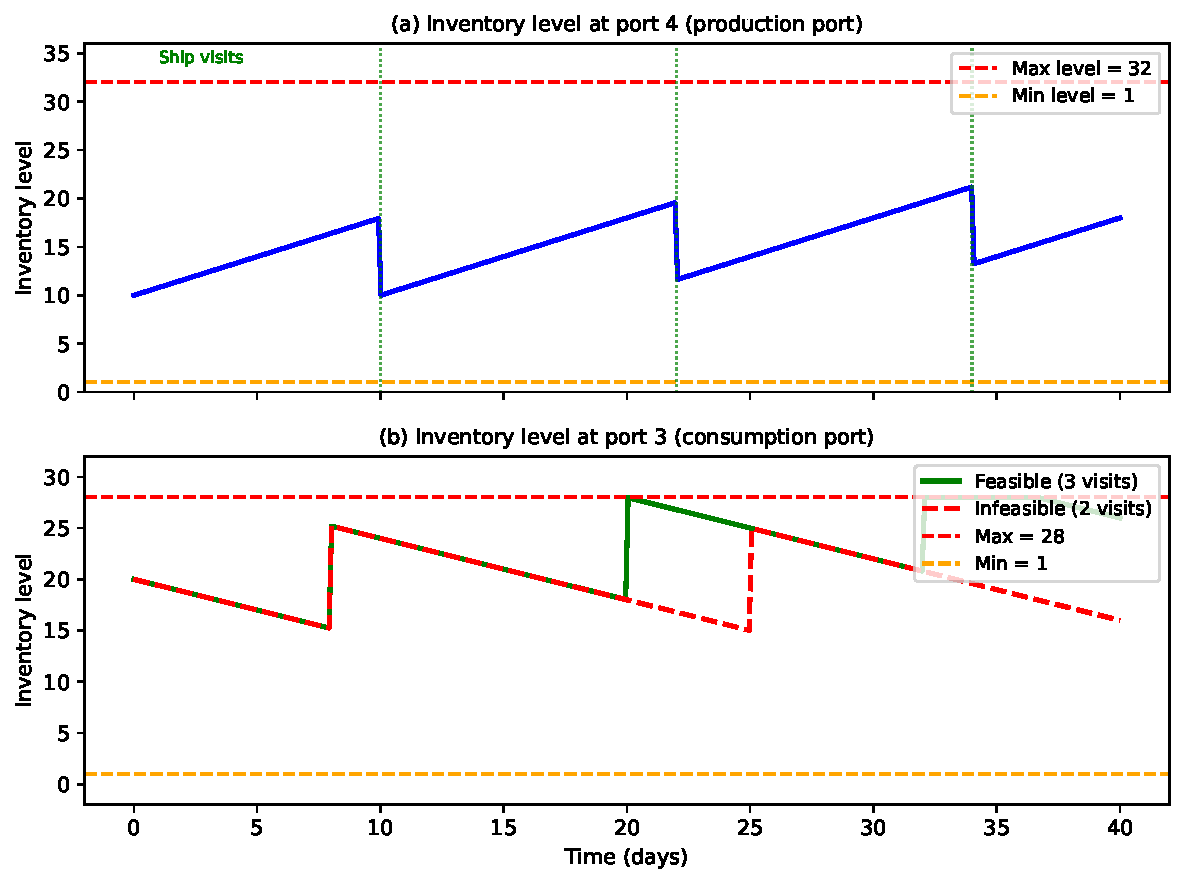
\includegraphics[width=0.78\textwidth]{inventory_levels.pdf}
    \caption{Top panel: inventory at a production port rises between ship
             visits (green dotted lines) and drops at each visit.  The red
             dashed line is the tank maximum; the orange dashed line is the
             minimum.  Bottom panel: inventory at a consumption port.
             A feasible 3-visit schedule (green) keeps inventory within
             bounds; a 2-visit schedule (red dashed) causes a stock-out.}
  \end{figure>
\end{frame>

\begin{frame}[allowframebreaks]{13.3.2 MIR Mathematical Model (Equations 13.40--13.59)}
  The full MIR model is an extension of the MPDP model that adds
  inventory-balance constraints.  We describe the key groups of constraints.
  This is a significantly more complex model than the basic MPDP because
  it must simultaneously optimise ship routes, visit timing, and load
  quantities.

  \medskip
  \textbf{Sets and parameters:}
  \begin{itemize}
    \item $M_i = \{1, 2, \ldots, |M_i|\}$ --- ordered set of \textbf{visits}
          to port $i$ during the planning horizon (each visit is indexed by $m$).
    \item $M_{ik}$ --- subset of visits to port $i$ that could be performed
          by ship $k$.
    \item $w_{im} \in \{0,1\}$ --- equals 1 if visit slot $m$ at port $i$
          is \textbf{skipped} (no ship visits), 0 otherwise.
    \item $q_{imk} \geq 0$ --- quantity loaded/unloaded by ship $k$ at port
          $i$, visit $m$.
    \item $\underline{S}_i, \overline{S}_i$ --- minimum and maximum
          \textbf{inventory} (tank capacity bounds) at port $i$.
    \item $S_i^0$ --- \textbf{initial inventory} at port $i$ at the start of
          the planning horizon.
    \item $T_i^B$ --- minimum \textbf{time between} consecutive visits to port $i$
          (berth availability constraint).
  \end{itemize}

  \begin{block}{Coverage Constraint (13.41)}
    \begin{equation}
      \sum_{k \in K} \sum_{j \in N_k} \sum_{n \in M_{ik}} x_{imjnk} + w_{im} = 1
      \qquad \forall\, i \in N,\, m \in M_i
      \tag{13.41}
    \end{equation}
    Every visit slot $(i, m)$ is served by exactly one ship (in which case
    $x = 1$ and $w = 0$) or is skipped ($w = 1$, $x = 0$).
    Skipping a visit means that slot is unused; the inventory balance
    constraint will check whether this is feasible.
  \end{block>

  \begin{block}{Flow Conservation (13.42--13.44)}
    \begin{align}
      \sum_{j \in N_k} \sum_{n \in M_{jk}} x_{o(k)1jnk} &= 1
      \qquad \forall\, k \in K \tag{13.42} \\
      \sum_{i \in N_k} \sum_{n \in M_{ik}} x_{imjnk} - \sum_{i \in N_k} \sum_{n \in M_{jk}} x_{jnimk} &= 0
      \quad j \notin \{o(k), d(k)\} \tag{13.43} \\
      \sum_{i \in N_k} \sum_{n \in M_{ik}} x_{imd(k)1k} &= 1
      \qquad \forall\, k \in K \tag{13.44}
    \end{align}
    These three constraints are analogous to the standard flow-conservation
    equations in the MPDP: ship $k$ departs its origin once (13.42), enters
    and leaves every intermediate port-visit the same number of times (13.43),
    and arrives at its artificial destination once (13.44).
  \end{block>

  \begin{block}{Inventory Balance (13.52--13.53)}
    \begin{align}
      s_{i1} - R_i t_{i1} &= S_i^0 \qquad \forall\, i \in N \tag{13.52} \\
      s_{i,m-1} - \sum_{k \in K} I_i q_{i,m-1,k} + R_i (t_{im} - t_{i,m-1}) - s_{im} &= 0
      \qquad m \geq 2 \tag{13.53}
    \end{align}
    Constraint (13.52) initialises the inventory at the first visit.
    Constraint (13.53) tracks the inventory between consecutive visits:
    the inventory at visit $m$ equals the inventory after visit $m{-}1$
    (adjusted for loading/unloading $q$), plus the accumulation/consumption
    at rate $R_i$ over the inter-visit time $t_{im} - t_{i,m-1}$.
    Here $I_i = +1$ for production ports and $I_i = -1$ for consumption ports.
  \end{block>

  \begin{block}{Inventory Bounds (13.54--13.55)}
    \begin{align}
      \underline{S}_i \leq s_{im} &\leq \overline{S}_i
      \qquad \forall\, i \in N,\, m \in M_i \tag{13.54} \\
      \underline{S}_i \leq s_{im} - \sum_{k \in K} I_i q_{im|M_i|k} + R_i(T - t_{im}) &\leq \overline{S}_i
      \qquad m = |M_i| \tag{13.55}
    \end{align}
    The inventory must stay within $[\underline{S}_i, \overline{S}_i]$ at
    all times.  Constraint (13.55) checks the \emph{end-of-horizon} inventory
    to prevent the plan from running out of stock after the planning window.
  \end{block>

  \begin{figure}
    \centering
    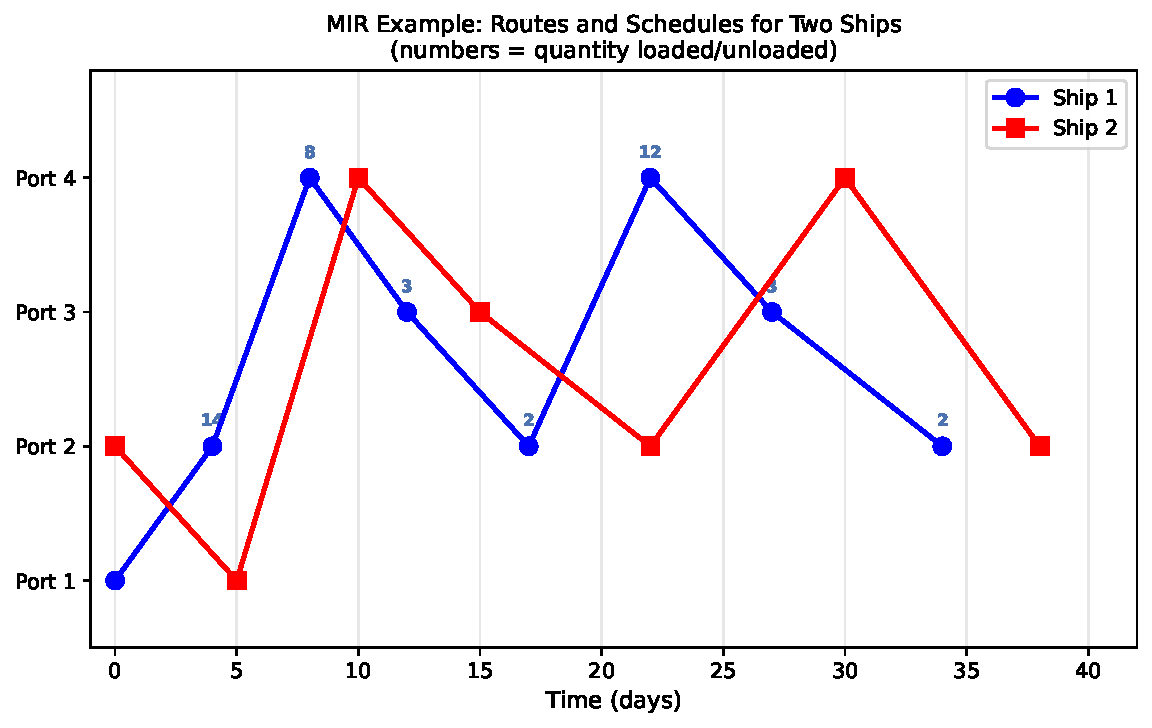
\includegraphics[width=0.72\textwidth]{mir_routes.pdf}
    \caption{Example MIR ship routes.  The horizontal axis is time (days);
             the vertical axis is port index.  Ship~1 (blue circles) and
             Ship~2 (red squares) visit ports in an interleaved pattern.
             Numbers at each dot indicate the quantity loaded or unloaded.
             The schedule must ensure inventory stays within $[\underline{S}_i,
             \overline{S}_i]$ at all times.}
  \end{figure>
\end{frame>

\begin{frame}[allowframebreaks]{MIR Solution Methods}
  The MIR model (13.40)--(13.59) is a large MIP.  On a time-space graph
  with 4 ports, 5 ships, and a 40-day planning horizon, the number of
  decision variables can exceed 100\,000.  Several solution approaches
  have been developed:

  \medskip
  \begin{block}{Arc-Flow vs.\ Path-Flow Formulations}
    The model described above is an \textbf{arc-flow} formulation ---
    it uses binary variables $x_{imjnk}$ for individual arcs between
    port-visits.  An alternative is the \textbf{path-flow} formulation,
    which uses continuous variables $\lambda_r$ representing the fraction
    of time a complete ship \emph{schedule} (sequence of all visits) is used.
    Path-flow formulations have tighter LP relaxations and are well-suited to
    column generation, but the pricing subproblem (finding the best ship
    schedule) is itself a complex shortest-path problem.
  \end{block>

  \begin{block}{Heuristics for MIR}
    \begin{itemize}
      \item \textbf{Decomposition}: first determine \emph{how many} visits
            each port needs (a simpler single-port problem), then solve a
            smaller routing problem.
      \item \textbf{Rolling horizon}: solve the MIR over a short window
            (e.g., 2 weeks), fix the first week's decisions, roll forward.
      \item \textbf{Column generation}: generate ship schedules (columns)
            that cover a feasible sequence of port visits, with inventory
            implications computed implicitly.
      \item \textbf{Adaptive Large Neighbourhood Search (ALNS)}: destroy
            and repair sub-schedules of ships while checking inventory
            feasibility.
    \end{itemize}
    Papageorgiou, Cheon, and Nemhauser \cite{PapGeorgiou2014} develop a
    branch-and-cut algorithm that solves the MIR model for up to 6 ports
    and 2 ships to optimality; Hvattum and Fagerholt (2010) show that
    rolling-horizon heuristics can provide near-optimal solutions for
    much larger instances.
  \end{block>

  \begin{figure}
    \centering
    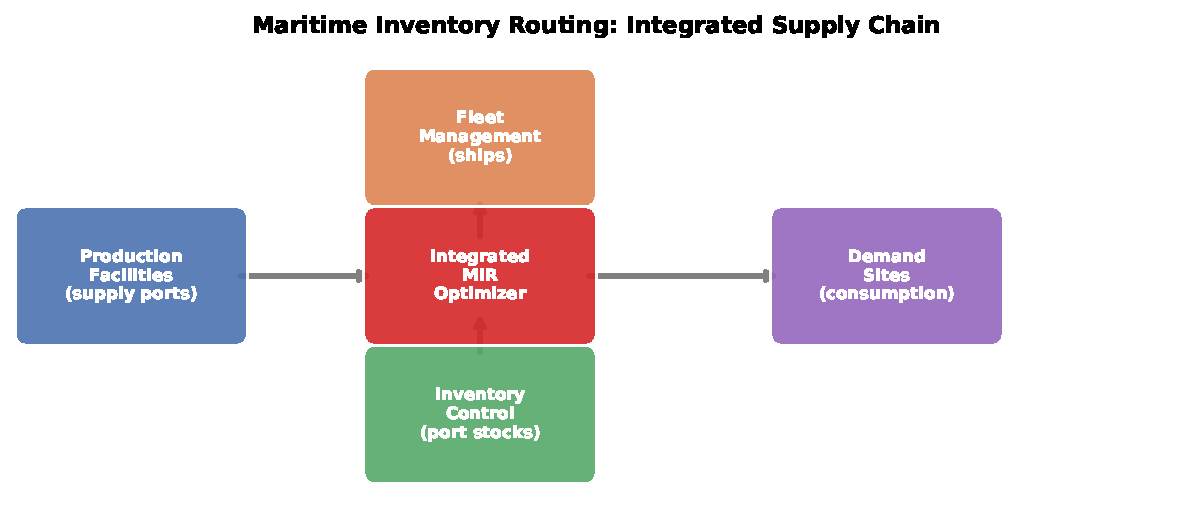
\includegraphics[width=0.72\textwidth]{supply_chain.pdf}
    \caption{The MIR optimizer integrates three traditionally separate
             decisions: production scheduling at supply ports (blue),
             fleet management (orange), and inventory control at demand
             ports (green).  The central optimizer balances all three
             simultaneously to minimise total cost.}
  \end{figure>

  \begin{alertblock}{Key Insight: MIR Captures the Full Supply-Chain Cost}
    Traditional ship routing models minimise \emph{shipping cost} alone.
    MIR additionally accounts for the cost of \emph{holding inventory}
    (capital tied up in stock), the cost of \emph{lost production} from
    stock-outs, and the cost of \emph{excess inventory} (spoilage,
    storage fees).  Studies show that MIR solutions can reduce total
    supply-chain cost by 5--15\% compared with separately optimising
    routing and inventory.
  \end{alertblock>
\end{frame>

%%%%%%%%%%%%%%%%%%%%%%%%%%%%%%%%%%%%%%%%%%%%%%%%%%%%%%%%%%%%%%%%%%%%%%%%%%%
\section{Dynamic and Stochastic Ship Routing}
%%%%%%%%%%%%%%%%%%%%%%%%%%%%%%%%%%%%%%%%%%%%%%%%%%%%%%%%%%%%%%%%%%%%%%%%%%%

\begin{frame}[allowframebreaks]{Section 13.4: Dynamic and Stochastic Ship Routing}
  All the models described so far assume that all information is
  \textbf{known in advance}: cargo locations, vessel positions, travel
  times, port availability.  In reality, ship routing is subject to
  many sources of uncertainty:

  \begin{itemize}
    \item \textbf{Weather uncertainty}: storms can delay a ship by several
          days on long ocean routes; fuel consumption spikes in heavy seas.
    \item \textbf{Port congestion and closure}: ports can be closed for
          unexpected maintenance, strikes, or tidal restrictions.
    \item \textbf{Spot market dynamics}: new cargo offers arrive
          continuously in real time; accepting them requires immediate
          re-routing.
    \item \textbf{Demand uncertainty}: in MIR settings, the consumption
          rate at a port may fluctuate with seasons, economic activity,
          or equipment failures.
  \end{itemize}

  \medskip
  \begin{block}{Two Paradigms for Handling Uncertainty}
    \begin{enumerate}
      \item \textbf{Dynamic (online) routing}: the plan is re-optimised
            each time new information arrives (``event-driven'' re-planning).
            This is a \emph{rolling horizon} or \emph{online optimisation}
            approach.
      \item \textbf{Stochastic programming}: uncertainty is modelled
            explicitly via probability distributions and scenario trees.
            The optimiser makes \emph{robust} decisions that perform
            well across all scenarios.
    \end{enumerate}
  \end{block>

  \begin{figure}
    \centering
    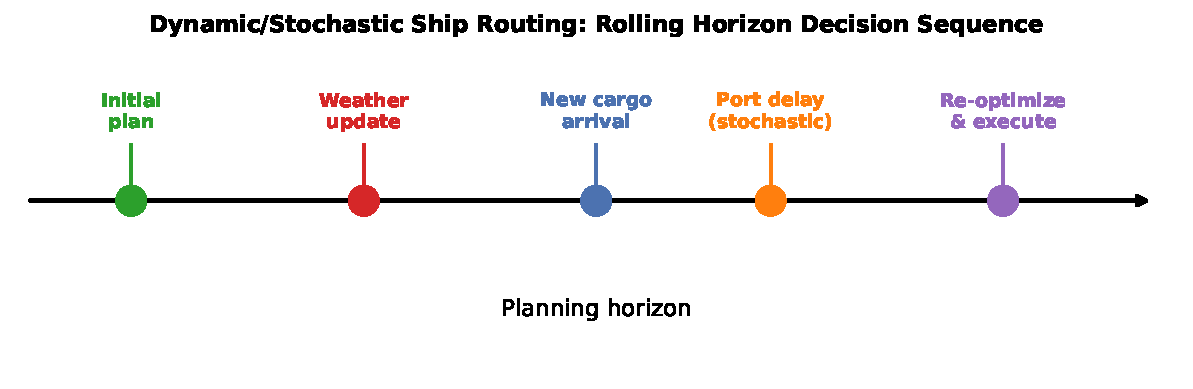
\includegraphics[width=0.72\textwidth]{dynamic_timeline.pdf}
    \caption{Rolling horizon decision sequence.  The planner re-optimises
             at each decision point (circle), accounting for new information
             (weather update, cargo arrival, port delay).  Only the first
             portion of the new plan is executed before the next
             re-optimisation.}
  \end{figure>
\end{frame>

\begin{frame}[allowframebreaks]{13.4.1 Dynamic Ship Routing: Rolling Horizon Approach}
  The most widely used practical approach to dynamic routing is the
  \textbf{rolling horizon} (also called \emph{model predictive control}
  in engineering).  The idea is simple:

  \medskip
  \begin{block}{Rolling Horizon Algorithm}
    \begin{enumerate}
      \item At decision time $t$, gather all currently known information:
            positions of ships, confirmed cargoes, weather forecasts,
            port status.
      \item Solve the static MPDP or MIR over a planning horizon
            $[t, t + H]$ (where $H$ is the horizon length, e.g., 3 weeks).
      \item \textbf{Execute} only the first $\delta$ time units of the
            resulting plan (e.g., the next 3 days of decisions are binding).
      \item At time $t + \delta$, receive new information (new cargo offers,
            updated weather, port closures), and re-solve the model.
      \item \textbf{Repeat} until the end of the planning period.
    \end{enumerate>
  \end{block>

  The \textbf{key design choices} in rolling horizon are:
  \begin{itemize}
    \item \textbf{Horizon length $H$}: too short $\Rightarrow$ myopic decisions
          (may miss a profitable cargo arriving 4 weeks away); too long
          $\Rightarrow$ expensive to re-solve and the far future is
          very uncertain.
    \item \textbf{Look-ahead $\delta$}: how far into the future the plan
          is committed before the next re-optimisation.
    \item \textbf{How to handle tail uncertainty}: some approaches add an
          ``end-of-horizon'' correction term to the objective to avoid
          artificially good tail decisions.
  \end{itemize}

  \medskip
  Tirado et al.\ (2013) apply a rolling horizon heuristic based on ALNS
  to a dynamic industrial shipping problem and report solutions within
  3--8\% of a perfect-information (clairvoyant) optimum even with high
  levels of spot-cargo uncertainty.

  \begin{exampleblock}{Worked Example: Rolling Horizon in Action}
    Suppose we manage 3 ships and a 30-day planning horizon ($H = 30$ days),
    with commitment horizon $\delta = 7$ days.

    \medskip
    \textbf{Day 0}: We solve the static MPDP for days 0--30.
    The plan assigns Ship~1 to Cargo~A (depart day 2, arrive day 9),
    Ship~2 to Cargo~B (depart day 1, arrive day 8), and reserves Ship~3
    for optional cargoes.

    \medskip
    \textbf{Day 7}: During the first 7 days, a new spot cargo~C appears
    (valued at \$200k; pickup day 10, delivery day 20) and Cargo~B's
    destination port is closed until day 12.  We re-solve the MPDP for
    days 7--37, incorporating these updates.  The new plan routes Ship~2
    directly to an alternative port and assigns Ship~3 to Cargo~C.

    \medskip
    The first 7 days of the new plan are binding; Ship~3 begins
    its voyage to Cargo~C's pickup port.

    \textbf{Key insight}: the rolling horizon framework handles dynamic
    cargo offers and disruptions naturally --- the planner simply
    re-solves with updated data at each period.
  \end{exampleblock>
\end{frame>

\begin{frame}[allowframebreaks]{13.4.2 Stochastic Ship Routing: Scenario-Based Optimisation}
  A more principled treatment of uncertainty uses \textbf{stochastic
  programming}, which models the future explicitly as a probability
  distribution over \emph{scenarios}.

  \medskip
  \begin{block}{Two-Stage Stochastic Programme}
    Let $\Omega$ (Omega) be the set of scenarios, and let $p_\omega$
    (p sub $\omega$ (omega)) be the probability of scenario $\omega$.
    The two-stage stochastic formulation is:
    \begin{equation}
      \max_{x \in X} \; c^\top x + \sum_{\omega \in \Omega} p_\omega Q(x, \omega)
    \end{equation}
    where $x$ is the \textbf{first-stage} (``here-and-now'') decision
    (made before uncertainty is revealed --- e.g., which cargoes to commit
    to), $X$ is the feasible set of first-stage decisions, and
    $Q(x, \omega)$ is the \textbf{second-stage} (``wait-and-see'') optimal
    value given first-stage decisions $x$ and scenario $\omega$
    (e.g., actual route adjustments after seeing weather).

    The term $\sum_{\omega} p_\omega Q(x, \omega)$ is the
    \textbf{expected recourse cost}: the average cost of adjusting the
    first-stage plan once the uncertainty is revealed.
  \end{block>

  \begin{alertblock}{How to Read This Formula}
    The formula says: choose first-stage decisions $x$ (commit to certain
    cargoes today) to maximise the sum of first-stage reward and expected
    future reward.  This is like deciding today whether to book a cargo
    contract (at a fixed price) knowing that tomorrow's weather may force
    you to reroute.  The stochastic programme balances the value of the
    contract against the expected extra cost of the reroute.
  \end{alertblock>

  \begin{figure}
    \centering
    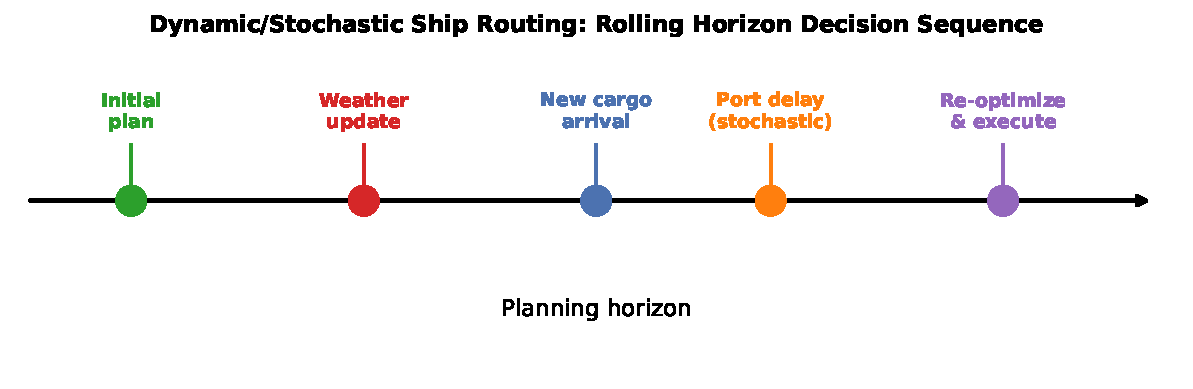
\includegraphics[width=0.60\textwidth]{dynamic_timeline.pdf}
    \caption{A rolling horizon view of stochastic ship routing.
             At each decision node, the planner sees a branching tree of
             future scenarios (weather states, cargo offers, port availability)
             with associated probabilities.  The stochastic programme
             finds first-stage decisions that are robust across all branches.}
  \end{figure>

  \begin{block}{Value of the Stochastic Solution (VSS)}
    A standard way to measure the benefit of stochastic modelling is the
    \textbf{Value of the Stochastic Solution (VSS)}:
    \begin{equation}
      \mathrm{VSS} = z^{SP} - z^{EV}
    \end{equation}
    where $z^{SP}$ is the objective value of the stochastic programme and
    $z^{EV}$ is the objective value of the \emph{expected-value} (EV)
    solution --- the solution obtained by replacing all random quantities
    with their expected values and solving a deterministic problem.

    If VSS $> 0$, the stochastic model provides real benefit.  Empirically,
    VSS for ship routing problems tends to be 5--15\% of the deterministic
    objective, meaning explicitly modelling uncertainty saves 5--15\% of
    costs compared with using mean-value inputs.
  \end{block>

  \begin{block}{Computational Challenge}
    The stochastic programme is much harder to solve than the deterministic
    version.  If there are $|\Omega|$ scenarios, the problem size grows
    linearly in $|\Omega|$.  For realistic instances with hundreds of
    scenarios, special techniques are needed:
    \begin{itemize}
      \item \textbf{Scenario reduction}: select a subset of $K$ representative
            scenarios (using distance-based clustering) that approximates the
            full distribution.
      \item \textbf{Sample Average Approximation (SAA)}: sample $N$ scenarios
            from the distribution and solve the resulting deterministic
            problem, then average across multiple SAA samples to estimate the
            true stochastic optimum.
      \item \textbf{Progressive hedging}: a Lagrangian decomposition method
            that solves one sub-problem per scenario and iteratively adjusts
            multipliers to achieve consensus on first-stage decisions.
    \end{itemize>
  \end{block>
\end{frame>

\begin{frame}[allowframebreaks]{13.4.2 Applications: Weather Routing and Port Disruptions}
  The chapter highlights two main application areas for stochastic ship
  routing models.

  \medskip
  \begin{block}{Weather Routing}
    Ocean weather strongly affects transit time and fuel consumption.
    A ship encountering a force-8 storm may experience a delay of
    1--3 days and an increase in fuel consumption of 30--50\% above
    calm-sea values.  Weather routing models typically:
    \begin{enumerate}
      \item Obtain a probabilistic weather forecast (wind, wave height,
            current) over the planning horizon.
      \item Model ship speed and fuel consumption as functions of
            wave height (via polar diagrams from the ship's specification).
      \item Optimise the route (waypoints) to balance transit time,
            fuel cost, and risk of damage or delay.
    \end{enumerate>
    Lo and Liu \cite{LoLiu2007} model the weather routing problem using a
    stochastic dynamic programme over a discretised ocean grid.  The optimal
    route may intentionally \emph{deviate} from the great-circle (shortest-distance)
    path to avoid a storm, saving more in fuel and delay than the extra
    distance costs.
  \end{block>

  \begin{block}{Stochastic Port Availability}
    Port congestion and berth availability are inherently stochastic:
    a berth might be unavailable because a previous ship ran over its
    slot, or a strike is called with no warning.  Modelling port
    availability as a random variable $\xi_{ik} \in \{0, 1\}$ (xi sub $i$-$k$,
    where 1 means the berth is available when ship $k$ arrives) leads to a
    chance-constrained programme:
    \begin{equation}
      \mathbb{P}\bigl(t_{ik} \in [\underline{T}_{ik}, \overline{T}_{ik}]
      \text{ and berth is available}\bigr) \geq 1 - \epsilon
    \end{equation}
    where $\epsilon$ (epsilon) is the acceptable probability of a time-window
    violation (e.g., $\epsilon = 0.05$ for a 5\% risk of missing the window).
    This formulation enforces \emph{probabilistic} time-window compliance
    rather than hard deterministic windows.
  \end{block>
\end{frame>

%%%%%%%%%%%%%%%%%%%%%%%%%%%%%%%%%%%%%%%%%%%%%%%%%%%%%%%%%%%%%%%%%%%%%%%%%%%
\section{Conclusions and Future Research}
%%%%%%%%%%%%%%%%%%%%%%%%%%%%%%%%%%%%%%%%%%%%%%%%%%%%%%%%%%%%%%%%%%%%%%%%%%%

\begin{frame}[allowframebreaks]{Section 13.5: Conclusions and Future Research Directions}
  \begin{block}{Summary of Chapter 13}
    This chapter has surveyed the rich landscape of ship routing and
    scheduling problems, covering three main problem classes:
    \begin{enumerate}
      \item \textbf{Cargo Routing and Scheduling (MPDP)}: assigning cargoes
            to ships and optimising each ship's route and schedule.
            Exact methods (branch-and-price) solve medium instances;
            metaheuristics (ALNS, tabu search) handle large real fleets.
      \item \textbf{Maritime Inventory Routing (MIR)}: simultaneously
            optimising ship routes and port inventory levels.  This integrated
            approach reduces total supply-chain cost by 5--15\% compared
            with decoupled optimisation.
      \item \textbf{Dynamic and Stochastic Routing}: handling weather,
            port congestion, and real-time cargo offers via rolling-horizon
            re-optimisation and stochastic programming.
    \end{enumerate}
  \end{block>

  \begin{block}{What Makes Maritime Routing Distinctive}
    Compared with classical road VRP, maritime ship routing presents
    unique challenges and opportunities:
    \begin{itemize}
      \item \textbf{Variable speed}: ships can trade time for fuel cost
            with a cubic relationship, adding a continuous decision layer
            absent in road VRP.
      \item \textbf{Enormous cargo quantities}: a single voyage decision
            can move 100\,000+ tonnes and generate millions in revenue,
            making optimality extremely valuable.
      \item \textbf{Long planning horizons}: weeks to months, rather than
            hours to days, leading to time-expanded graph models and
            rolling-horizon methods.
      \item \textbf{Integration with supply chains}: MIR integrates
            production planning, shipping, and inventory control in a way
            that has no direct analogue in road logistics.
      \item \textbf{Environmental impact}: ships produce 2--3\% of global
            CO$_2$ emissions; route and speed optimisation directly reduces
            carbon footprint.
    \end{itemize}
  \end{block>

  \begin{alertblock}{Future Research Directions}
    The chapter identifies several open challenges at the research frontier:
    \begin{enumerate}
      \item \textbf{Larger and more realistic MIR models}: current exact
            methods solve instances with 4--6 ports; real supply chains
            involve 20--50 ports.  Better decompositions and tighter
            formulations are needed.
      \item \textbf{Dynamic MIR}: combining the real-time re-planning
            capability of dynamic routing with the inventory-tracking
            power of MIR remains an open problem.
      \item \textbf{Integrated speed optimisation}: few papers jointly
            optimise routes, cargo assignment, \emph{and} speed profiles;
            this three-way integration is computationally challenging.
      \item \textbf{Environmental objectives}: incorporating carbon
            emissions, sulphur caps, and emission control areas as
            hard constraints or additional objectives.
      \item \textbf{Autonomous shipping}: as autonomous ships become
            viable, the decision-making authority shifts to on-board
            computers, requiring real-time algorithms that can solve
            routing problems at sea with incomplete information.
    \end{enumerate>
  \end{alertblock>

  \begin{block}{Key References}
    \begin{itemize}
      \item Christiansen, Fagerholt, Nygreen, Ronen (2007): comprehensive
            survey of maritime transportation OR.
      \item Fagerholt, Gausel, Rakke, Ronen (2010): variable-speed
            optimisation for ship routing.
      \item Papageorgiou, Cheon, Nemhauser (2014): branch-and-cut for MIR.
      \item Tirado, Hvattum, Fagerholt, Cordeau (2013): heuristics for
            dynamic stochastic industrial shipping.
      \item St\aa lhane, Andersson, Christiansen, Cordeau, Desaulniers (2012):
            branch-and-cut for routing with split loads.
    \end{itemize}
  \end{block>
\end{frame>

%%%%%%%%%%%%%%%%%%%%%%%%%%%%%%%%%%%%%%%%%%%%%%%%%%%%%%%%%%%%%%%%%%%%%%%%%%%
\section{Python Implementation}
%%%%%%%%%%%%%%%%%%%%%%%%%%%%%%%%%%%%%%%%%%%%%%%%%%%%%%%%%%%%%%%%%%%%%%%%%%%

\begin{frame}[fragile]{Python: Greedy Tramp Routing Heuristic}
\begin{lstlisting}[caption={Greedy construction heuristic for the tramp pickup-and-delivery problem.
                             This implements the insertion-based procedure described in Section 13.2.}]
import math, itertools

def haversine_nm(lat1, lon1, lat2, lon2):
    """Great-circle distance in nautical miles."""
    R = 3440.065  # Earth radius in nm
    phi1, phi2 = math.radians(lat1), math.radians(lat2)
    dphi = math.radians(lat2 - lat1)
    dlam = math.radians(lon2 - lon1)
    a = math.sin(dphi/2)**2 + math.cos(phi1)*math.cos(phi2)*math.sin(dlam/2)**2
    return 2*R*math.asin(math.sqrt(a))

def fuel_cost(distance_nm, speed_kn=14.0, alpha=0.002, fuel_price=600):
    """Total fuel cost (USD) for a leg, using cubic F(v)=alpha*v^3."""
    days = distance_nm / (speed_kn * 24)   # sailing time in days
    tonnes = alpha * speed_kn**3 * days    # total fuel (tonnes)
    return tonnes * fuel_price

class Cargo:
    def __init__(self, cid, pickup, delivery, qty, revenue, mandatory=True):
        self.cid, self.pickup, self.delivery = cid, pickup, delivery
        self.qty, self.revenue, self.mandatory = qty, revenue, mandatory
        self.spot_cost = revenue * 1.5  # cost if covered by spot ship

class Ship:
    def __init__(self, kid, origin, capacity):
        self.kid, self.origin, self.capacity = kid, origin, capacity
        self.route = [origin]  # sequence of (lat,lon) positions
        self.load = 0.0

def greedy_insertion(ships, cargoes):
    """
    Greedy construction: assign cargoes to ships one at a time,
    choosing the assignment that maximises marginal profit.
    """
    unassigned = list(cargoes)
    assignments = {s.kid: [] for s in ships}
    spot_market = []

    # Sort by mandatory first, then by revenue descending
    unassigned.sort(key=lambda c: (-int(c.mandatory), -c.revenue * c.qty))

    for cargo in unassigned:
        best_gain, best_ship = -math.inf, None
        for ship in ships:
            current_load = sum(c.qty for c in assignments[ship.kid])
            if current_load + cargo.qty > ship.capacity:
                continue  # capacity violation
            # Marginal cost: distance to pickup + distance pickup->delivery
            last_pos = ship.origin if not assignments[ship.kid] \
                       else assignments[ship.kid][-1].delivery
            d1 = haversine_nm(*last_pos, *cargo.pickup)
            d2 = haversine_nm(*cargo.pickup, *cargo.delivery)
            marginal_cost = fuel_cost(d1) + fuel_cost(d2)
            gain = cargo.revenue * cargo.qty - marginal_cost
            if gain > best_gain:
                best_gain, best_ship = gain, ship

        if best_ship is not None:
            assignments[best_ship.kid].append(cargo)
            print(f"  Cargo {cargo.cid} -> Ship {best_ship.kid} "
                  f"(net gain = ${best_gain:,.0f})")
        else:
            spot_market.append(cargo)
            print(f"  Cargo {cargo.cid} -> SPOT market "
                  f"(cost = ${cargo.spot_cost:,.0f})")

    total_cost = sum(c.spot_cost for c in spot_market)
    total_revenue = sum(c.revenue * c.qty
                        for s in ships for c in assignments[s.kid])
    print(f"\nTotal revenue: ${total_revenue:,.0f}")
    print(f"Spot market cost: ${total_cost:,.0f}")
    print(f"Net profit: ${total_revenue - total_cost:,.0f}")
    return assignments, spot_market

# ── Example: 4 cargoes, 2 ships ──────────────────────────────
if __name__ == '__main__':
    ships = [
        Ship('S1', (51.9, 4.5),  60000),  # Rotterdam, cap 60kt
        Ship('S2', (1.3, 103.8), 50000),  # Singapore, cap 50kt
    ]
    cargoes = [
        Cargo('C1', (51.9,4.5),  (29.9,-90.0), 55000, 8.0, mandatory=True),
        Cargo('C2', (1.3,103.8), (22.3,114.2), 40000, 6.5, mandatory=True),
        Cargo('C3', (29.9,-90.0),(51.9,4.5),   30000, 7.0, mandatory=False),
        Cargo('C4', (22.3,114.2),(35.7,139.7), 45000, 9.0, mandatory=False),
    ]
    greedy_insertion(ships, cargoes)
\end{lstlisting}
\end{frame}

\begin{frame}[fragile]{Python: Inventory Level Simulation (MIR)}
\begin{lstlisting}[caption={Simulation of port inventory levels under a given ship schedule.
                             This illustrates the inventory balance constraints (13.52)--(13.53).}]
import numpy as np
import matplotlib
matplotlib.use('Agg')
import matplotlib.pyplot as plt

def simulate_inventory(port, rate, s0, s_min, s_max, visit_times, quantities, T=40):
    """
    Simulate inventory level at a single port over [0, T] days.

    Parameters
    ----------
    port    : port name (for plotting)
    rate    : production rate (>0) or consumption rate (<0), units/day
    s0      : initial inventory level at t=0
    s_min   : minimum allowed inventory (tank floor)
    s_max   : maximum allowed inventory (tank ceiling)
    visit_times : list of ship visit times (days)
    quantities  : list of quantities loaded (+) or unloaded (-) at each visit
    T       : planning horizon (days)
    """
    # Build piecewise-linear trajectory
    t_points = [0.0] + sorted(visit_times) + [float(T)]
    s_points = [s0]

    s_current = s0
    for idx, t in enumerate(sorted(visit_times)):
        dt = t - (sorted(visit_times)[idx-1] if idx > 0 else 0)
        s_current += rate * dt            # accumulate / deplete
        s_points.append(s_current)        # inventory just before visit
        s_current += quantities[idx]      # apply load/unload at visit
        s_points.append(s_current)        # inventory just after visit

    # Add final point
    dt_final = T - (sorted(visit_times)[-1] if visit_times else 0)
    s_points.append(s_current + rate * dt_final)
    t_points_ext = [0.0]
    for t in sorted(visit_times):
        t_points_ext += [t, t]
    t_points_ext.append(T)

    # Check feasibility
    feasible = all(s_min <= s <= s_max for s in s_points)
    print(f"Port {port}: {'FEASIBLE' if feasible else 'INFEASIBLE'}")
    print(f"  Inventory range: [{min(s_points):.1f}, {max(s_points):.1f}]")
    print(f"  Allowed range:   [{s_min}, {s_max}]")
    return t_points_ext, s_points, feasible

# ── Example: Port 4 (production) and Port 3 (consumption) ──
t4, s4, ok4 = simulate_inventory(
    port='4 (Production)',
    rate=+0.8,   # produces 0.8 units/day
    s0=10, s_min=1, s_max=32,
    visit_times=[10, 22, 34],
    quantities=[-8, -8, -8]   # ship unloads 8 units each visit
)
t3, s3, ok3 = simulate_inventory(
    port='3 (Consumption)',
    rate=-0.6,   # consumes 0.6 units/day
    s0=20, s_min=1, s_max=28,
    visit_times=[8, 20, 32],
    quantities=[+10, +10, +10]  # ship delivers 10 units each visit
)
\end{lstlisting}
\end{frame}

%%%%%%%%%%%%%%%%%%%%%%%%%%%%%%%%%%%%%%%%%%%%%%%%%%%%%%%%%%%%%%%%%%%%%%%%%%%
\section{Summary and Bibliography}
%%%%%%%%%%%%%%%%%%%%%%%%%%%%%%%%%%%%%%%%%%%%%%%%%%%%%%%%%%%%%%%%%%%%%%%%%%%

\begin{frame}[allowframebreaks]{Chapter Summary: Key Concepts and Take-aways}
  This chapter has presented ship routing and scheduling as a rich family
  of combinatorial optimisation problems with significant real-world
  impact.  Here are the most important ideas to carry forward.

  \medskip
  \begin{block}{Core Message 1: Three Shipping Modes, Three Problem Classes}
    Industrial, liner, and tramp shipping each give rise to fundamentally
    different optimisation problems.  Tramp and industrial shipping lead to
    MIP-based pickup-and-delivery models; liner shipping leads to network
    design problems.  Maritime Inventory Routing bridges shipping and
    production planning.
  \end{block>

  \begin{block}{Core Message 2: The MIP Model Captures the Essential Structure}
    The MPDP model (13.1)--(13.15) is the fundamental building block.
    All extensions --- split loads, variable speed, compartments, stochastic
    elements --- augment this base model with additional variables and
    constraints.  Understanding the base model deeply makes all extensions
    accessible.
  \end{block>

  \begin{block}{Core Message 3: Column Generation is the Workhorse Solver}
    For medium-to-large instances, branch-and-price (combining B\&B with
    column generation) is the standard exact method.  It avoids exponential
    enumeration by generating only ``useful'' ship routes.  For very large
    or dynamic instances, ALNS and tabu search provide high-quality
    solutions efficiently.
  \end{block>

  \begin{block}{Core Message 4: Uncertainty Requires Explicit Treatment}
    Weather, port disruptions, and real-time cargo offers make ship routing
    inherently dynamic.  Rolling-horizon re-optimisation is the most
    practical approach; stochastic programming provides theoretically
    stronger guarantees at higher computational cost.
  \end{block>

  \begin{alertblock}{Connection to Other VRP Chapters}
    Ship routing is not an isolated domain.  It inherits the pickup-and-delivery
    structure from Chapter~8, the column-generation methodology from
    Chapter~6, the metaheuristic framework from Chapters~4--5, and
    the stochastic modelling from Chapter~10.  The maritime setting
    provides an especially rich application where all these techniques
    combine.
  \end{alertblock>
\end{frame>

\begin{frame}[allowframebreaks]{Selected Bibliography}
  \begin{thebibliography}{99}
    \bibitem{CFR2004}
    M.\ Christiansen, K.\ Fagerholt, and D.\ Ronen,
    \emph{Ship routing and scheduling: Status and perspectives},
    Transportation Science, 38 (2004), pp.\ 1--18.

    \bibitem{CFNR2007}
    M.\ Christiansen, K.\ Fagerholt, B.\ Nygreen, and D.\ Ronen,
    \emph{Maritime transportation},
    in C.\ Barnhart and G.\ Laporte (eds.), \textit{Handbooks in Operations
    Research and Management Science}, Vol.\ 14, 2007, pp.\ 189--284.

    \bibitem{Fagerholt2010}
    K.\ Fagerholt, G.\ Gausel, J.\ G.\ Rakke, and H.\ N.\ Ronen,
    \emph{Maritime routing and speed optimisation with emission control areas},
    Transportation Research Part C, 52 (2015), pp.\ 57--73.

    \bibitem{PapGeorgiou2014}
    D.\ J.\ Papageorgiou, G.\ Cheon, and G.\ L.\ Nemhauser,
    \emph{Approximate dynamic programming for a class of long-horizon
    maritime inventory routing problems},
    Transportation Science, 49 (2015), pp.\ 870--883.

    \bibitem{Tirado2013}
    G.\ Tirado, L.\ M.\ Hvattum, K.\ Fagerholt, and J.-F.\ Cordeau,
    \emph{Heuristics for dynamic and stochastic routing in industrial shipping},
    Computers \& Operations Research, 40 (2013), pp.\ 253--263.

    \bibitem{Stalh2012}
    M.\ St\aa lhane, H.\ Andersson, M.\ Christiansen, J.-F.\ Cordeau, and
    G.\ Desaulniers,
    \emph{A branch-and-cut method for a ship routing and scheduling problem
    with split loads},
    Computers \& Operations Research, 39 (2012), pp.\ 3361--3375.

    \bibitem{LoLiu2007}
    H.\ K.\ Lo and C.\ W.\ Liu,
    \emph{Adaptive ship routing through stochastic ocean currents:
    General formulations and empirical results},
    Transportation Research Part B, 41 (2007), pp.\ 6--24.

    \bibitem{Vidal2007}
    J.\ Vidal,
    \emph{CO$_2$ output from shipping twice as much as airlines}, 2007.
    Available at \url{http://www.guardian.co.uk}.

    \bibitem{UNCTAD2011}
    UNCTAD,
    \emph{Review of maritime transport}, 2011,
    United Nations, New York and Geneva.
  \end{thebibliography}
\end{frame>

\end{document}
